\subsection{Pruebas unitarias del algoritmo en simulaci\'on de mapas 1} % (fold)
\label{sub:subsection name1}
    Para la realizaci\'on de un programa, es necesario realizar las
        pruebas unitarias correspondientes para comprobar el
        funcionamiento de cada una de las partes involucradas con el
        programa.
    \vskip 0.5cm
    En la realizaci\'on de las pruebas unitarias, se utiliz\'o Google
        Test, el cual es un framework de Google que funciona parael lenguaje de programaci\'on C++, que es el lenguaje
        utilizado para el desarrollo del simulador del Physarum. Es
        importante recordar que las pruebas unitarias son las que se
        encargan de verificar que cada una de las partes que
        componen a un software funcionen bien una a una, por lo
        que el mayor uso que se le di\'o al framework es la realizaci\'on
        de las pruebas unitarias al c\'odigo del simulador del
        Physarum, verificando cada una de las funciones que lo
        componen y dem\'as componentes del software.
    \vskip 0.5cm
    Principalmente, fue probado la implementaci\'on del
        algoritmo, el cual contiene algunas funciones importantes y
        algunas otras que devuelven valores importantes para la
        correcta implementaci\'on del algoritmo.
    \vskip 0.5cm
    Algunas de las pruebas unitarias que fueron aplicadas son las
    siguientes:
    \vskip 0.5cm
    %figrura
    \begin{figure}[htbp]
        \centering
        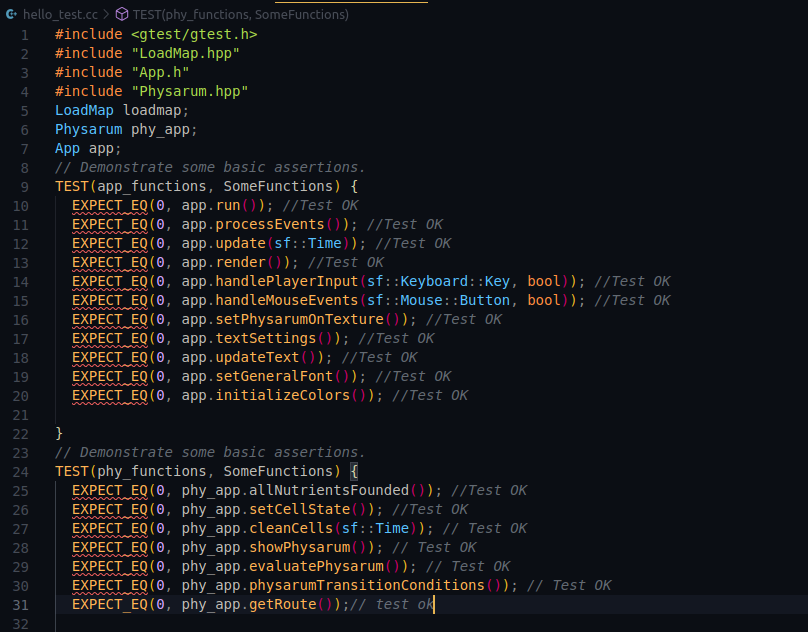
\includegraphics[width=0.5\textwidth]{./images/Pruebas/simulador/image007.png}
        \caption{Prueba unitaria 1}
        \label{fig:Prueba unitaria 1}
    \end{figure}
    \vskip 0.5cm
    Como se puede ver, gran parte de las pruebas realizadas al
        algoritmo fueron satisfactorias a este punto, por lo que
        podemos ver que a pesar de que la implementaci\'on fue en su
        mayor\'ia correcta, hay una peque\~na ventana de oportunidad
        para la mejora y correcci\'on de la implementaci\'on del
        algoritmo en determinadas circunstancias, donde a pesar de
        que casi toda la implementaci\'on no est\'a relacionada a una entrada del usuario, sino a partes involucradas en la
        realizaci\'on de la simulaci\'on, entonces hay muy pocos casos
        en los que una parte de este mismo falle, ya que, debido a la
        implementaci\'on de las reglas, la manera en la que funciona
        un aut\'omata celular y del propio funcionamiento del
        algoritmo en s\'i, no es permitido que algo falle ya que esto
        alterar\'ia completamente el resultado final del algoritmo,
        realizando c\'alculos err\'oneos en la simulaci\'on y errando el
        objetivo del algoritmo.
% subsection subsection name (end)